\chapter{Implementation}
\label{chap:basics}

After discussing the most important design aspects of the honeypot system, we now implemented a prototype that can simulate a basic environment and might help gather information about an attacker's intentions. 

\section{Overview}
The following diagram illustrates the final pipeline that handles commands.

%\begin{figure}[H]
   % \centering
    %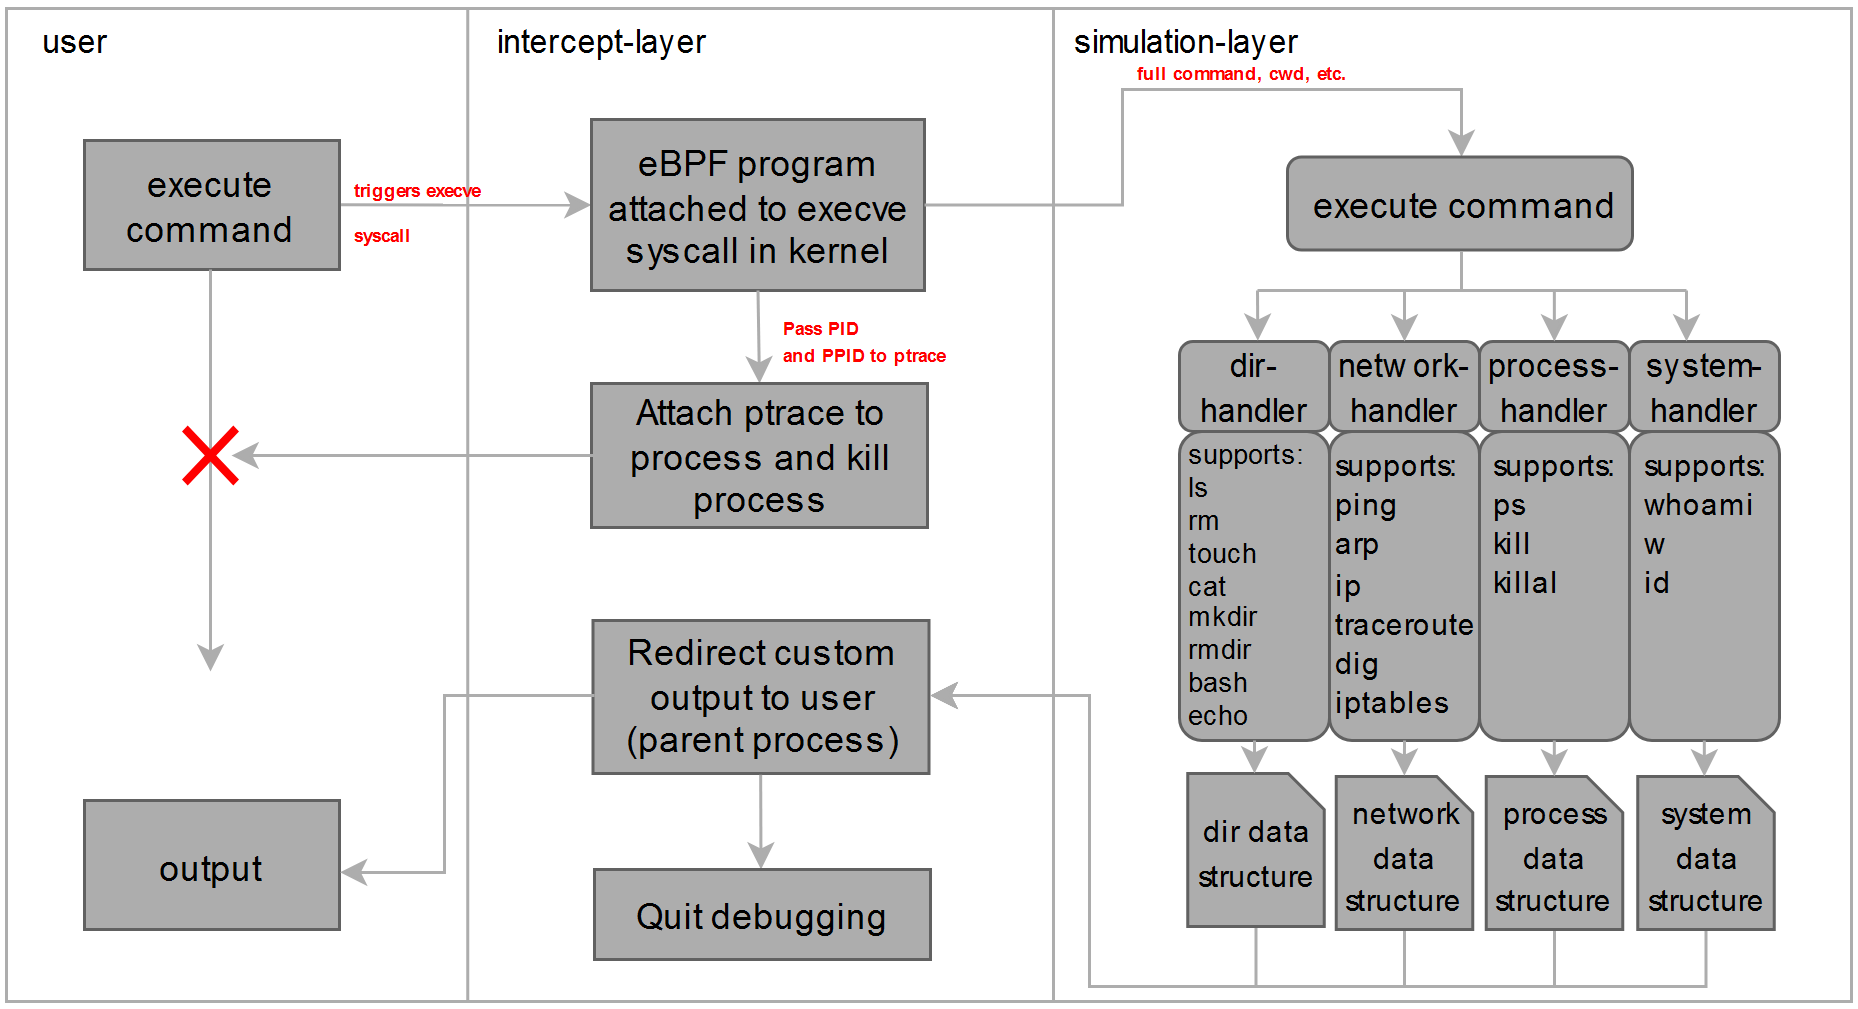
\includegraphics[width=1\linewidth]{bilder/pipeline.PNG}
    %\caption{Command pipeline}
    %\label{fig:enter-label}
%\end{figure}

\begin{figure}[H]
    \centering
    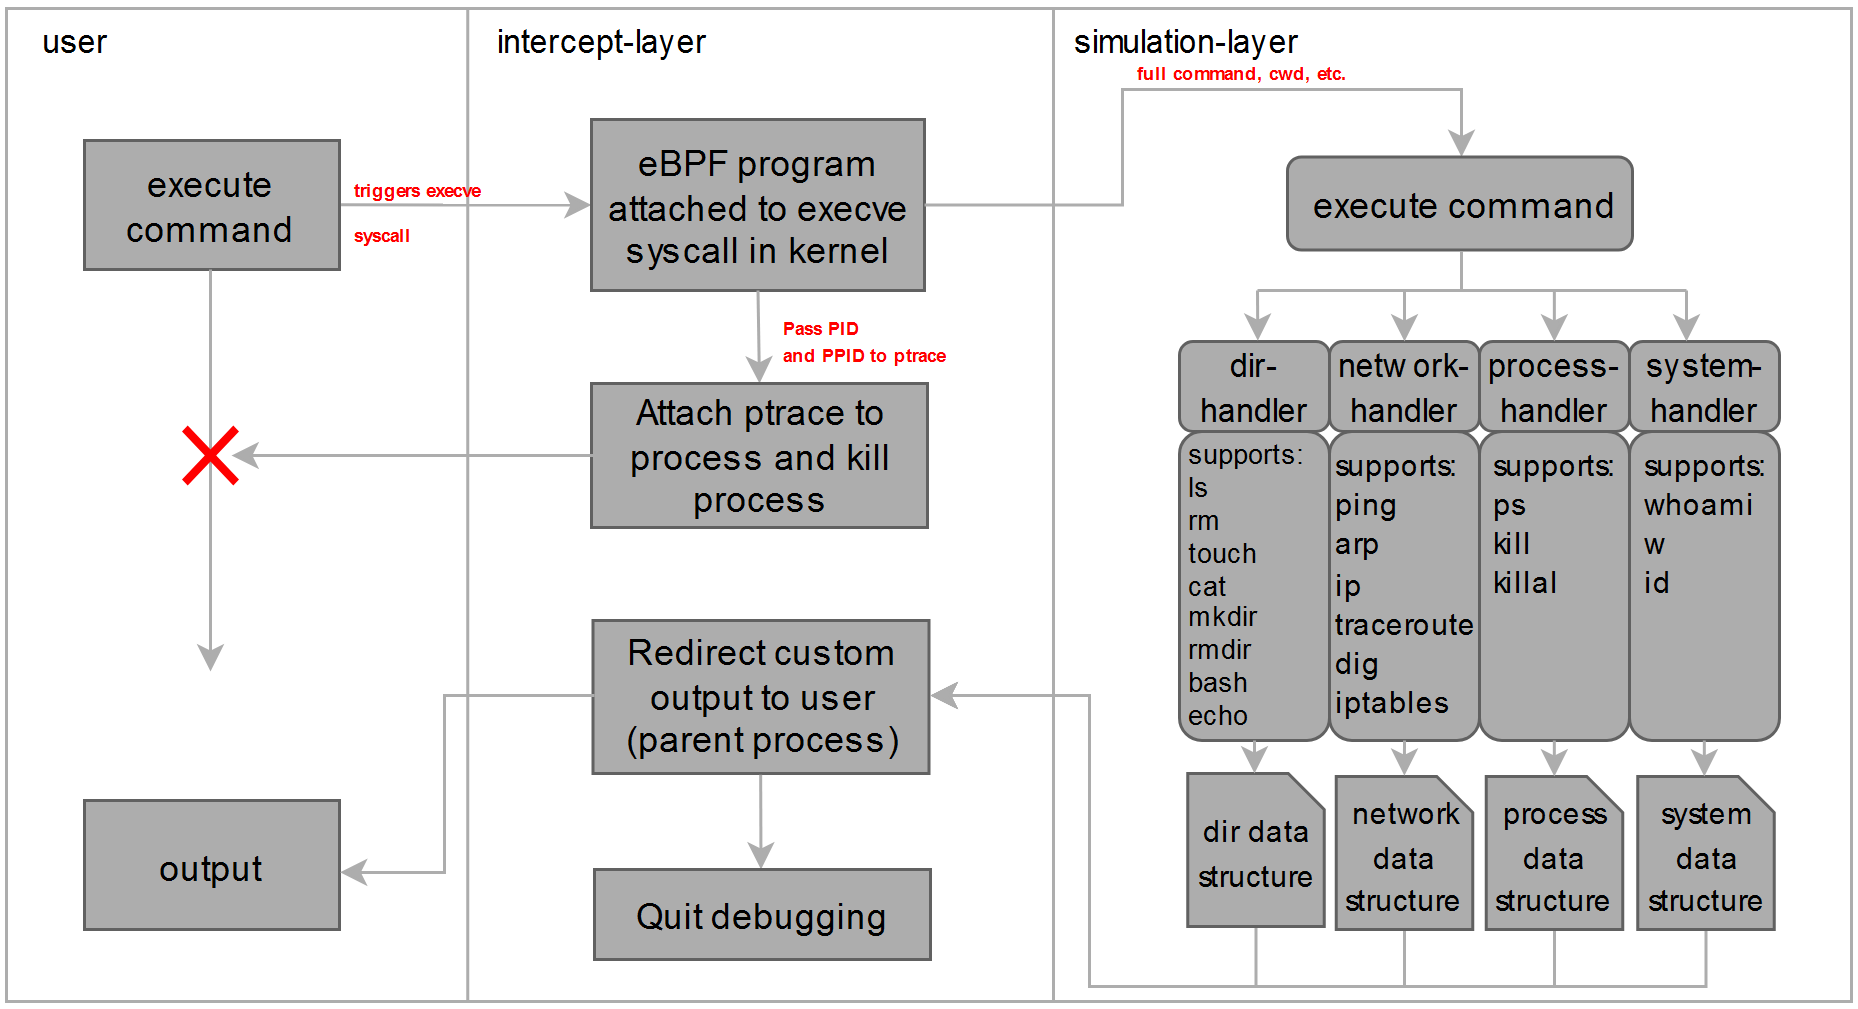
\includegraphics[width=1\linewidth]{bilder/pipeline.PNG}
    \caption{Command pipeline}
    \label{fig:enter-label}
\end{figure}


As shown in the graph, we use an intercept-layer to block the immediate execution of a command that is provided by a user. This layer is capable of calling APIs and deciding, which type of command it just intercepted. It can distinguish between directory-commands, network-commands, process-commands and system-commands. Examples for the different classes will be shown later.
After intercepting a command, it will call the corresponding API and deliver the command itself, all provided arguments and the current directory as a payload.

In the next step, the four handlers act as API endpoints and can react to a given input. For example a user might execute the ls-command. The "dir-handler" generates a simulated file system on program start using the data structure and can therefore apply a simulated ls-command on the virtual file system. The output is returned to the calling intercept-layer which will present it to the user. In theory the interception of commands and the simulated output can not be detected by the user.

\section{Command intercept}
As described in the previous section, the intercept-layer has two basic tasks. On the one hand, it has to trace and intercept all commands a user wants to execute. These commands have to be classified according to the four categories we defined (directory, network, process, system) and the corresponding API has to be called. On the other hand, the output of the called API has to be presented to the user in a way he can not distinguish it from a real output of the system.
\subsection{Tracing commands via eBPF}
\label{sub:ebpf}
To trace commands that are issued by the user we implemented and modified a eBPF program based on the exemplary "execsnoop.py" program that comes with the python bcc library \cite{execsnoop}. This program enables us to trace execution details of the "execve" system call that is triggered once the user commands are executed. Within the c-based eBPF program we use a structure to collect data such as the process ID, the parent process ID, the user id, the actual command as well as the arguments and other details like the return value. Furthermore, the user identifier 1000 of the user that is traced by the honeypot is hardcoded into the eBPF program. 
\begin{lstlisting}
# Define BPF program
bpf_text = """
#include <uapi/linux/ptrace.h>
#include <linux/sched.h>
#include <linux/fs.h>

#define ARGSIZE  128
#define UID_FILTER 1000

enum event_type {
    EVENT_ARG,
    EVENT_RET,
};

struct data_t {
    u32 pid;  
    u32 ppid; 
    u32 uid;
    char comm[TASK_COMM_LEN];
    enum event_type type;
    char argv[ARGSIZE];
    int retval;
};
\end{lstlisting}
To store events that can be read from userspace we make use of a BPF map.
\begin{lstlisting}
BPF_PERF_OUTPUT(events);    
\end{lstlisting}
Within the eBPF program we also utilize a function "syscall\_\_execvee" to trace the "execve" system call and capture the already mentioned parameters and store them in the BPF map. Helper functions such as "\_\_submit\_arg" and "submit\_arg" are responsible for reading and submitting arguments towards the map. Using the "BPF" class we then initialize the implemented eBPF program.
\begin{lstlisting}
b = BPF(text=bpf_text)
\end{lstlisting}
Afterwards, the function name of the "execve" system call needs to be resolved since these names can vary depending on the underlying kernel version. This ensures that we are tracing the correct system call.
\begin{lstlisting}
execve_fnname = b.get_syscall_fnname("execve")  
\end{lstlisting}
We then attach the eBPF program to the system call by utilizing bcc's "attach\_kprobe" which will execute the prior defined function "syscall\_\_execvee" once the "execve" system call is triggered.
\begin{lstlisting}
b.attach_kprobe(event=execve_fnname, fn_name="syscall__execve")
\end{lstlisting}
Lastly, we also attach a "kretprobe" which will capture returns of the system call and then execute the defined "do\_ret\_sys\_execve" eBPF function which simply captures the return value of the system call. 
\begin{lstlisting}
b.attach_kretprobe(event=execve_fnname, fn_name="do_ret_sys_execve")
\end{lstlisting}
All of the prior mentioned code samples are implemented within the main program "jamjar.py". Whenever the system call is triggered we execute the same routine which is implemented within the "proc\_event" function. This function processes the data that is returned by the eBPF program and therefore parses the process ID, which is required to intercept and kill the processes as well as the full commands which are needed for generating the fake output that is later returned to the user. Note that the "ptrace" debugger is attached to the target process as soon as the process ID has been parsed. Since the simulation layer also requires other data such as the current working directory for the command issued by the user, we derive such details from the file system entries for the traced processes within "/proc/<pid>/cwd". 

\newpage

\begin{lstlisting}
def proc_event():
    event = b["events"].event(data)

    if event.type == EventType.EVENT_ARG:
        argv[event.pid].append(event.argv)
    elif event.type == EventType.EVENT_RET:
        target_process = attach_ptrace(event.pid)
        argv_text = b' '.join(argv[event.pid]).replace(b'\n', b'\\n')
        cwd = os.readlink(f"/proc/{event.pid}/cwd")
        tty = os.readlink(f"/proc/{event.pid}/fd/0").replace("/dev/","")
        username = pwd.getpwuid(event.uid).pw_name
        # Getting cleaned command
        full_command,cmd_wo_args = cleaup_cmd(event.comm,argv_text)

        # Print event to console
        print_event(full_command,cwd,event.uid)
        # Handle commands
        event_handler(cmd_wo_args,event.pid,full_command,cwd,tty,event.ppid,username,target_process)
\end{lstlisting}
Once all the required details are parsed they are passed to a function "print\_event" which simply prints information regarding the traced command to the screen for logging purposes.
\bild{bilder/logoutput.png}{JamJar console output}{JamJar console output}
Furthermore, the parsed data is also passed to the function "event\_handler" which is responsible to call different subroutines which are implemented within "Subroutines.py" depending on the type of command that was issued by the user differentiating between directory, network and process commands.
\begin{lstlisting}
match comm:
    case ("ls"|"rm"|"touch"|"cat"|"echo"):
        PtraceSubroutines.dir_routine(pid,ppid,full_cmd,cwd,target_process)
        DEBUGGER.quit()
    case ("ping"|"arp"|"ip"|"traceroute"|"dig"|"iptables"):
        PtraceSubroutines.network_routine(pid,ppid,full_cmd,target_process)
        DEBUGGER.quit()
    case ("ps"|"kill"|"killall"):
        PtraceSubroutines.process_routine(pid,ppid,full_cmd,tty,username,target_process)
        DEBUGGER.quit()
    case ("whoami"|"w"|"id"):
        PtraceSubroutines.system_routine(pid, ppid, full_cmd, username, target_process)
        DEBUGGER.quit()
\end{lstlisting}
To constantly monitor for system call events we make use of a simple while-loop which then calls the "proc\_event" function once an event is triggered.
\begin{lstlisting}
b["events"].open_perf_buffer(proc_event)
    while True:
        try:
            b.perf_buffer_poll()
        except KeyboardInterrupt:
            exit()
\end{lstlisting}

\subsection{Intercepting and Killing Processes}
As mentioned in the previous section, as soon as the process id for the traced command is parsed we make use of the "ptrace" python library to attach to said process and put it in a halted state. This is required since processes for the traced commands exit rather quickly. Once "ptrace" is utilized to attach to the target process and all the required details are parsed within "jamjar.py" we move into the subroutines for the different commands within "PtraceSubroutines.py". This is where we kill the processes for the commands issued by the user and also pass the details to the simulation layer to generate the fake data and return it to the user. The different routines for the directory, network and process commands are very similar with the exception of commands such as "ping" or "traceroute" as they require time intervals for different sequences of output that is returned to the user. To establish a basic understanding of such routines we now detail the routine for network commands "network\_routine".
This function is called and passed with the parameters process id (pid), the parent process id (ppid), the full command (command) and the ptrace context (running\_process). 
\begin{lstlisting}
def network_routine(pid,ppid,command,running_process):
    ...
\end{lstlisting}
To first retrieve the fake output, we invoke a call to the simulation layer passing the full command.
\begin{lstlisting}
    cmd_output = CMD.invoke_network(command)
\end{lstlisting}
Now that the fake data has been generated we make sure to verify if the returned data is of type list, this would be the case if we need to delay the output for commands such as "ping" or "traceroute". If this is the case, we then call the helper function "write\_to\_proc" for each item in the list with a delay of one second. The helper function "write\_to\_proc" simply writes the fake output to the parent process of the issued user command which in this case is the tty of the user that issued the command.  
\begin{lstlisting}
    if type(cmd_output) == list:
            for n,item in enumerate(cmd_output):
                write_to_proc(item+"\n",str(ppid))
                if n < 5:
                    time.sleep(1)
        # Write modified output to target process
        else:
            write_to_proc(check_linebreak(cmd_output),str(pid))
        kill_and_quit(running_process,str(pid))
\end{lstlisting}
Once the fake output is returned to the user, we then call our second helper function\\ "kill\_and\_quit" which takes the "ptrace" context for the target process to then kill said process by sending a signal "SIGTERM". This then concludes the process of the intercept layer to trace and intercept user commands.

\newpage

\begin{lstlisting}
def kill_and_quit(process,pid):
    # Kill the process using SIGTERM
    process.kill(signal.SIGTERM)
    print(f"\t\\--> Attached to process [{pid}] and killed it!")    
\end{lstlisting}

\subsection{Challenges and Takeaways}
While implementing the intercept layer we came across multiple challenges. Originally we had in mind to perform this whole process by utilizing only eBPF programs. eBPF generally seems to be mainly used for its tracing capabilities and is therefore not meant to write within the kernel or modify system call return values and behavior to provide security within the kernel \cite{bcc}. Though it seems to be possible in certain edge cases it is not recommended as it would require changing certain kernel configurations which would put the availability of the operating system at risk.\\
While we opted to implement the actual interception and the termination of the processes via "ptrace" we originally attached to the command processes within "PtraceSubroutines.py" as it looked more reasonable at the time. This lead to the issue of race conditions as the processes for the user commands oftentimes already finished executing before we were able to attach to them. Therefore we decided to attach and halt the process as soon as we parsed the process ID via eBPF, this minimized the occurrence of race conditions significantly. Nevertheless, race conditions are still relevant as an attacker could simply use programs written in compiler languages such as C to outrun the execution flow of our python implemented honeypot.\\ Finally, we managed the termination of the user command processes by sending the "SIGTERM" signal. This would normally return signal messages such as "Terminated" to the user which would indicate that something went wrong while executing the command. To solve this we turned off the monitor mode for the target user by disabling it within the user's bash profile ".bashrc".
\begin{lstlisting}
export PROMPT_COMMAND='set +m'    
\end{lstlisting}


\newpage

\section{Command handler}
Next we have a look at the four command handlers.
As already mentioned in the theory-chapter, we can distinguish between four types of commands.
\textbf{Directory} related commands, \textbf{Network} related commands, \textbf{Process} related commands and \textbf{System} related commands.
Each command corresponds to a dedicated handler in the python code:
\begin{itemize}
    \item Directory-commands -> dir\_handler
    \item Network-commands -> network\_handler
    \item Process-commands -> process\_handler
    \item System-commands -> system\_handler
\end{itemize}

Each handler acts as an API-endpoint and needs some context to "execute" commands.
All four handlers define and build a simulated environment that can be used to execute the commands.
This environment is semi-persistent.
This means it is generated in a pre-defined state at program start and is completely discarded once the program stops.
So in case it is broken, all that has to be done is restart the program.
This could also be done periodically, for example every hour.

\subsection{Directory}
Simulating a directory is the most challenging part of the three handlers.
The most crucial aspect is designing a file system that on the one hand provides all the information that might be needed if a user executes a command (e.g \texttt{ls -a}).
On the other hand, commands like \texttt{rm} alter the file system, which needs to be taken into account and tracked. Further more, this simulated file system has to be efficient, as a delay of the output might be suspicious to an adversary.

To simulate the filesystem, we use Python objects.
Basis is the class \textbf{file}, which is used to represent a single "virtual" file.
Each file object has several attributes, such as permissions, owner and name.
One key aspect is the attribute "parent", which can be used to reference the parent object (a directory) of a file.
The init-method provides some default-values each time a new object of the class "File" is generated.

Directories can be seen as a special kind of files, because they share a lot of the same attributes.
Therefore we defined a new class "Dir" in "dir.py" which extends the class "File".
It also adds a new attribute to all objects of the class which is called "content".
This content-attribute holds a dictionary of all files and directories that are currently located in the directory.
In this case the key of the dictionary is the name of the object, the value is the object itself.
We used this approach to store the content rather than a simple list, because it allows for a quick and efficient navigation through the simulated fileystem. 

The last file that is needed before we focus on the directory-handler is called "helper.py".
This file contains helper-methods for all four handlers.
For example the method "create-fake-dir-data-helper" is used to create an initial fake directory structure with some data.
The dir-handler itself will call this function on initialization and set its root-point to the root of the generated fake file system.

Currently there are eight directory-commands with some common arguments supported.

\begin{table}[H]
    \centering
    \begin{tabular}{c|c|c}
        Command & Description & Supported Arguments\\
        \hline 
        ls & list directory contents & a / l / r\\
        rm & remove files or directory & r / f\\
        touch & create file or change file timestamp & -\\
        cat (see ch. \ref{sub:cat}) & list file content & -\\
        echo (see ch. \ref{sub:echo}) & displays text or command output & -\\
        mkdir & create directory & -\\
        rmdir & remove directory & -\\
        cd (see ch. \ref{sub:cd}) & change directory & -\\
    \end{tabular}
    \caption{Currently supported directory-commands}
    \label{tab:my_label}
\end{table}

Each command has a source-directory, where it is executed from (passed from the interception layer), and a target-directory (extracted from the command), where the command should be executed. Here are some examples:

\begin{table}[H]
    \centering
    \begin{tabular}{c|c|c}
        Command & Source directory & Target directory\\
        \hline
        user@comp:~\$ ls & /home/user & /home/user \\
        user@comp:~\$ ls /etc & /home/user & /etc \\
        user@comp:/home ls user & /home & /home/user \\
    \end{tabular}
    \caption{Possible context of the command "ls"}
    \label{tab:my_label}
\end{table}

Because of the many possible ways to execute a simple command such as \texttt{ls}, we have to think of a way to extract different sections of a command in a way that it is represented in a unified structure that can then be used to get the desired output.
The \texttt{ls} command for example can be split into four main points of interest:

\texttt{\color{blue}ls \color{red}-al \color{green}/home/user} executed in \texttt{\color{orange}/home}

\begin{enumerate}
    \item The command itself (\texttt{\color{blue}ls})
    \item Optional arguments (\texttt{\color{red}-al})
    \item Optional path. Can be an absolute or a relative path (\texttt{\color{green}/home/user})
    \item The directory the command was executed in (\texttt{\color{orange}/home})
\end{enumerate}

%%\todo[inline]{Zu viele Farben?}

Each of these sections, can hold a variety of different inputs, which change the output of the command.
Therefore, we need to look at each section and act accordingly.

To simplify this process, we first look at what variables are needed at the end to decide the output of the command.

For \texttt{ls} they are:

\begin{enumerate}
    \item The source directory
    \item The target directory
\end{enumerate}

With these two variables, we can always walk through the filesystem and find the directory the user wants to see.

By definition, every intercepted command is handed over with the source-directory as a parameter. Therefore this is fixed and can be used to find out the target-directory.
In the easiest case, the command does not contain a target-directory, meaning we can set the src-dir as the target-dir.
In case there is a parameter given as the target-directory, we are only interested in the object that represents the last folder in the given path.
For example, if the target-directory is given as \texttt{/a/b/c/d}, we only need the object of \texttt{d} to access its attributes like the "content", containing a dictionary of all files in that virtual folder.
To achieve this, the following small algorithm is used:

\begin{lstlisting}
for layer in src_dir_list:
    src_obj = src_obj.content[layer]
\end{lstlisting}

This algorithm on the virtual structure allows for an easy and efficient usage of the virtual file system.

If every aspect of the command has been taken into account, it is easy to determine the expected output.
For example if we know the source and target object of an ls command, we can find the corresponding object in our data-structure, which holds the desired data.
Finally the content of this object must be returned:

\begin{lstlisting}
for file in target_obj.content:
    output += file + " "
\end{lstlisting}

Additionally at this point further instructions and arguments that alter the display of the output would be taken into account.
This could for example be reversing the output string in case of the "-r" argument being present in the command.

Likewise when using the data-structure and helper functions to dissect a command, implementing further commands like \texttt{rm} and \texttt{touch} is very straight forward.

For example when using the data-structure and correct preprocessing of the command, a file can be deleted like the following.
This, of course, only represents the simplest case without any checks and arguments.

\begin{lstlisting}
src_obj.content.pop(target_file)
\end{lstlisting}

\begin{figure}[H]
    \centering
    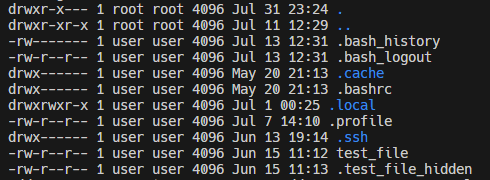
\includegraphics[width=1\linewidth]{bilder/ls.png}
    \caption{Simulated output of "ls -al /home/user"}
\end{figure}

\subsection{Network}
Currently there are six network-commands with some common arguments supported.

\begin{table}[H]
    \centering
    \begin{tabular}{c|c|c}
        Command & Description & Supported Arguments\\
        \hline 
        ip & interface related information & a / r / add / del\\
        ping & ping a host & c \\
        arp & view arp entries & d\\
        traceroute & see routers in the route to a host & - \\
        dig & retrieve DNS records for domains & x / v / A / AAAA\\
        iptables (see ch. \ref{sub:iptables}) & manage Linux network traffic rules & L / h / A / D / F\\
    \end{tabular}
    \caption{Currently supported network-commands}
    \label{tab:my_label}
\end{table}

On startup of the program we have to create a fake arp-table as well as a fake list of interfaces. This information is currently hard-coded but could be semi-randomized in the future. When the program is started, the methods "create-fake-arp-data-helper" and "create-fake-interface-data-helper" are execute which load the initial values for the arp-table and the list of interfaces from the file "interface.py" and "arp.py". After that, the environment is ready to handle network commands.

As already mentioned, we currently support the commands \texttt{ping}, \texttt{arp}, \texttt{ip}, \texttt{traceroute}, \texttt{dig} and \texttt{iptables} with some flags that are used often by a malicious actor.

On execution of the ping-command, our program will first check whether an ip-address is given as a parameter or a domain name. In the easiest case, an ip-address is given. The program will check, whether this ip-address is located in the same subnet as the the simulated interfaces using the python-library "ipcalc". If it is in the same subnet, the output of a normal ping-command will be handed back using a random value for the roundtriptime between 10 and 50 ms for each ping. By default, four pings are sent, but the user can adjust this number with the -c flag, specifying the desired number of pings.

\begin{figure}[H]
    \centering
    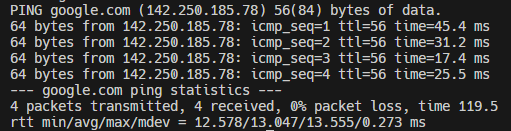
\includegraphics[width=1\linewidth]{bilder/ping.png}
    \caption{Simulated output of "ping google.com"}
\end{figure}

For each target that is pinged by the attacker, an entry in the arp-table should be established. Therefore we need to distinguish between local ip-adresses in the same subnet and addresses outside our subnet. If the ip-address is in the local subnet, an arp-entry for this ip-address is created. If the ip-address is outside the local network, an entry for the standard gateway is created.

The function also calculates realistic roundtrip time (RTT) statistics, including the minimum, average, maximum, and standard deviation of the RTT values. These computed statistics are displayed in the final output along with the RTT values for each individual ping.

Last but not least, if an attacker does not ping an ip-address but uses a domain name as a parameter, this address is translated into a real ip-address using the library "socket".

Similar to ping, traceroute shows information about the reachability of network devices, just with other faked data.

The arp-command can print the current arp-table or delete entries from this table. On startup, only the local address of the host is included in the arp-table. Whenever a user tries to ping a target as described in the previous section, this address is dynamically added to the arp-table. Of course these entries can also be deleted by the user.

The \textbf{ip} command is the most extensive command in the network handler.
It supports two \textbf{main arguments} which can be seen as two separate commands.

\begin{enumerate}
    \item \texttt{ip a}: Shows information about the network interface. 
    \item \texttt{ip r}: Shows information about set network routes.
\end{enumerate}

Both of these sub-commands support \texttt{add} and \texttt{del} as arguments.
Similar to the directory commands, a structure of objects is used in the back-end to store all necessary information about interfaces such as ip-address, gateway, hw-address, etc.

\begin{figure}[H]
    \centering
    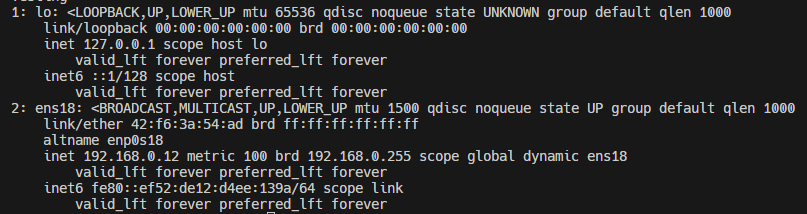
\includegraphics[width=1\linewidth]{bilder/ip.png}
    \caption{Simulated output of "ip a"}
\end{figure}

The \texttt{dig} command simulates the functionality of the widely used DNS querying tool, providing the ability to retrieve domain name system records and perform both forward and reverse lookups. The command accepts a domain name or IP address as input and processes it to generate a realistic DNS response. It supports a few flags to tailor the query, such as specifying whether to retrieve IPv4 (A) or IPv6 (AAAA) records or conducting reverse lookups for IP addresses.

When a domain name is queried, the program performs a forward lookup, resolving the name to its associated IP addresses. Depending on the flags used, the results include either IPv4 or IPv6 addresses, with simulated metadata such as TTL (Time To Live) and DNS query times. In cases where the domain cannot be resolved, the output indicates an appropriate error status, such as \textit{SERVFAIL}, replicating real-world DNS behavior. The generated response mirrors the typical output of the dig tool, including headers, sections for questions, answers, and additional information, along with metadata like the server address and the timestamp.

For reverse lookups, the command processes the provided IP address into the reverse DNS format (e.g., \textit{1.0.0.127.in-addr.arpa}) and attempts to resolve it back to a domain name. If the IP address can be resolved, the output includes a PTR record with the corresponding domain name. If the resolution fails, the result indicates a failure status, such as \textit{NXDOMAIN}, and includes relevant authority section data to simulate real-world behavior.

\begin{figure}[H]
    \centering
    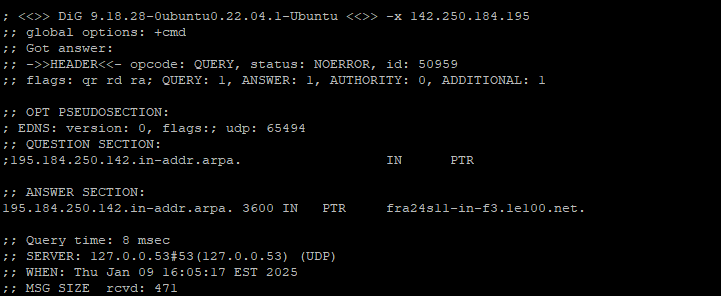
\includegraphics[width=1\linewidth]{bilder/rev-dns.png}
    \caption{Simulated output of "dig -x 142.250.184.195"}
\end{figure}


\subsection{Process}
Simulating process commands does also need a default list of simulated processes that run on the system. This initial list is copied from a running linux system in order to be as authentic as possible. Currently the process list with all its parameters is hard-coded but could be semi-randomized in the future. For example process-ids or cpu- and memory-usage could be given a random value on each program start. 

We identified the following commands to be important in an attack scenario: 

\begin{table}[H]
    \centering
    \begin{tabular}{c|c|c}
        Command & Description & Supported Arguments\\
        \hline 
        ps & Display processes & -a, -e, -A, -f, -C, -u, a, u, x \\
        kill, killall  & Terminate process & - \\
    \end{tabular}
    \caption{Currently supported process-commands}
    \label{tab:my_label}
\end{table}


%https://man7.org/linux/man-pages/man1/ps.1.html
The most difficult one to implement is \texttt{ps}. It reports a snapshot of the current processes.
The version of \texttt{ps} that is mimicked has three different syntax options: UNIX-options that can be grouped and use a dash in front of the letter; BSD options which also can be grouped but do not use a dash and GNU options that use two dashes\cite{noauthor_ps1_2024}.
Our implementation includes some Unix options and some BSD options. 

Every \texttt{ps} call from the intercept layer includes the current terminal and the current user ID. With this information an accurate representation of the processes can be generated and returned. Without a given parameter, \texttt{ps} hands back a list of all processes currently running by the user who executes the command and the current terminal the command is executed in\cite{noauthor_ps1_2024}. In our implementation all process objects are filtered by the user id (UID) and the terminal (TTY) that is send by the intercept layer:

\begin{lstlisting}
    if not args_str:
        for process in self.output: # none
            if (process.tty == tty or process.tty == "pts/0") 
            and process.uid == uid:
                processes.append(process)
\end{lstlisting}


The process objects that fit that criteria are selected and their information is turned into an output that looks similar to the original output using .format():

\begin{lstlisting}
    for process in processes:
        process_list.append([process.pid, process.tty, process.stat, 
        process.time[-4:], process.ucmd])

        process_list = [["PID", "TTY", "STAT", "TIME", "COMMAND"]] + 
        sorted(process_list, key=lambda x: x[0])

        for row in process_list:
             output+= "{:>6} {:<8} {:<4} {:<4} {:<4}\n".format(*row)
\end{lstlisting}

The process information that is presented by \texttt{ps} without a parameter includes the process ID (PID), the terminal associated with the process (TTY), the accumulated CPU time in [DD-]hh:mm:ss format (TIME) and the executable name (CMD)\cite{noauthor_ps1_2024}. As seen in Figure \ref{fig:outputps} the layout of the simulated output resembles the real output, but it is possible to manipulate the processes that are shown. The following options follow a similar algorithm simply changing the filtered attributes and the format of the output for each parameter. 

\begin{figure}[H]
    \centering
    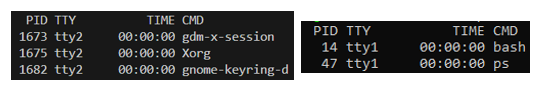
\includegraphics[width=1\linewidth]{bilder/real_and_fake_ps.png}
    \caption{Simulated output of "ps" (left) and real output (right)}
    \label{fig:outputps}
\end{figure}

The Unix options that are included in our implementation are "-a", "-e/-A", "-f", "-C" and "-u" and most combinations of multiple parameters. \texttt{ps -a} displays all processes but excludes all session leaders. Session leaders have the same process Id and Session ID. \texttt{ps -e}  or \texttt{ps -A} display all processes of the system without any filters. \texttt{ps -C} is able to filter all processes by the process name\cite{noauthor_ps1_2024}.

\begin{figure}[H]
    \centering
    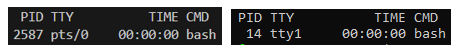
\includegraphics[width=1\linewidth]{bilder/real_and_fake_psC.png}
    \caption{Simulated output of "ps -C bash" (left) and real output (right)}
    \label{fig:enter-label}
\end{figure}

Another filter option is \texttt{ps -u}. This parameter filters all processes by a user Id and only displays processes belonging to that user\cite{noauthor_ps1_2024}.

The last Unix parameter that is implemented is "f". It is able to display additional information about the processes by adding additional columns. The information includes the user ID, process ID, parent process ID, CPU utilization in percent, terminal associated with the process, elapsed CPU utilization time for the process and the name of executable command\cite{noauthor_ps1_2024}.

\begin{figure}[H]
    \centering
    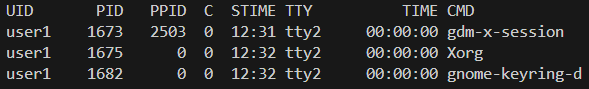
\includegraphics[width=1\linewidth]{bilder/fake_psf.png}
    \caption{Simulated output of "ps -f"}
    \label{fig:enter-label}
\end{figure}

This option only changes the format of the output and not the displayed selection of processes. It can also be combined with other parameters. For example it is possible combine "-f" and "-u" to search for a specific user ID and display the selected with more information as seen in Figure \ref{fig:outputpsuser}. 

\begin{figure}[H]
    \centering
    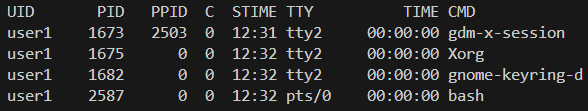
\includegraphics[width=1\linewidth]{bilder/fake_psfu.png}
    \caption{Simulated output of "ps -fu user1"}
    \label{fig:outputpsuserl}
\end{figure}

The BSD-options that are implemented include "a","x", "u". \texttt{ps a} displays all processes in the current terminal but has a different layout additionally displaying the process state codes (STAT) and the long name of the executable command \cite{noauthor_ps1_2024} as seen in Figure \ref{fig:outputpsa}. 

\begin{figure}[H]
    \centering
    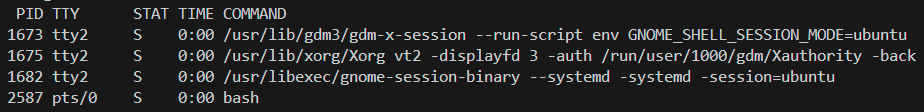
\includegraphics[width=1\linewidth]{bilder/fake_psa.png}
    \caption{Simulated output of "ps a"}
    \label{fig:outputpsa}
\end{figure}

The option \texttt{ps x} shows all processes of the current user, but combined with "a" it displays all processes in the system. The option "u" displays a user-oriented format with additional information like the used ID, cpu utilization of the process in "\#\#.\#" format, ratio of the process's resident set size to the physical memory on the machine, virtual memory size of the process in KiB, resident set size and the start time of the process. The popular combination of all three \texttt{ps aux} shows all processes with additional information \cite{noauthor_ps1_2024} as seen in Figure \ref{fig:fakepsaux}.

\begin{figure}[H]
    \centering
    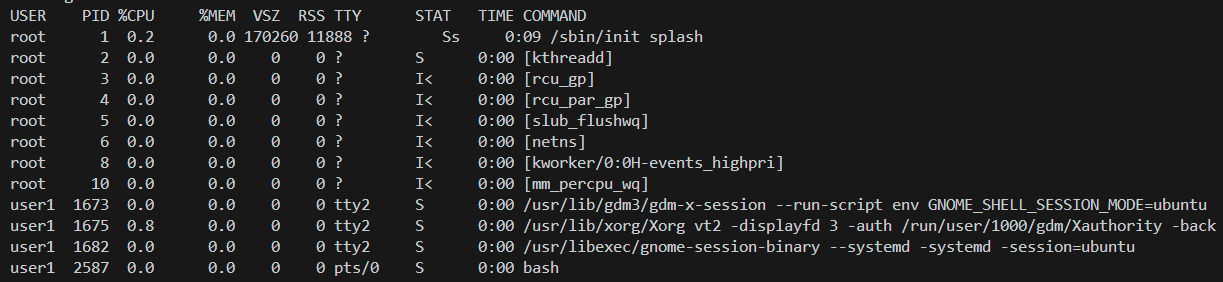
\includegraphics[width=1\linewidth]{bilder/fake_psaux.png}
    \caption{Simulated output of "ps aux"}
    \label{fig:fakepsaux}
\end{figure}

The commands \texttt{kill} and \texttt{killall} can used to terminate processes\cite{kill}\cite{noauthor_killall1_2023}. This is done by simply removing entries from the list of simulated processes. \texttt{kill} is used with a process ID to remove the process with this ID\cite{kill}.\texttt{killall} uses the executable command to terminate a process\cite{noauthor_killall1_2023}.

\begin{lstlisting}
for process in self.output:
            if process.pid == target_process:
                self.output.remove(process)
                valid_arg = True
\end{lstlisting}

To check weather the process was removed a \texttt{ps} command can be submitted before and after submitting \texttt{kill} or \texttt{killall}. If the argument is not valid an error message is displayed that resembles a real error message.

\subsection{System}
The system command handler is responsible for simulating common system-related commands such as \texttt{whoami}, \texttt{id}, and \texttt{w}. These commands are used to retrieve information about the current user and system status, often employed in reconnaissance or debugging scenarios. While their current implementation is hardcoded to provide consistent and predictable outputs, they could be extended in the future to include semi-randomized elements for greater realism.

Currently there are only three basic system-commands supported.

\begin{table}[H]
    \centering
    \begin{tabular}{c|c|c}
        Command & Description & Supported Arguments\\
        \hline 
        whoami & displays the current username & -\\
        id & shows user and group IDs & - \\
        w & lists active user session details & -\\
    \end{tabular}
    \caption{Currently supported system-commands}
    \label{tab:my_label}
\end{table}

The \texttt{whoami} command simply returns the current username, which is passed to the event handler upon initialization. The \texttt{id} command provides details about the user’s ID, group ID, and associated groups, with static values reflecting a typical Linux environment. The \texttt{w} command simulates an active session, displaying system uptime, load averages, and user activity, including login times, idle durations, and the currently executed command. Although the \texttt{w} command currently uses fixed data, attributes such as system uptime, load averages, or idle times could be randomized in the future to enhance authenticity.

\begin{figure}[H]
    \centering
    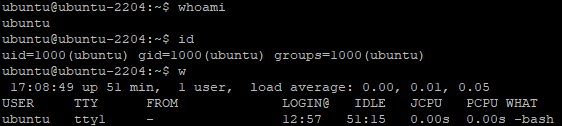
\includegraphics[width=1\linewidth]{bilder/system.png}
    \caption{Simulated output of system commands}
    \label{fig:enter-label}
\end{figure}

The underlying implementation relies on a unified interface for command execution. When a command is issued, the handler identifies the requested command, extracts the relevant parameters, and invokes the corresponding helper function to produce the simulated output. This modular approach allows for flexibility and extensibility, making it easy to add additional system commands in the future.

\section{Logging}
Every command intercepted and processed by the handlers is logged in a central log-file. This is done using the python-library "logging". The basic configuration of the logging is executed once on program startup. It is persistent, so even if the program ends and is run again, the new log entries will be appended to the existing file. It needs the following configuration parameters: \newline

\begin{itemize}
    \item level: Sets the threshold for this logger. Messages which are less severe than the given level, in this case "INFO", will be ignored. Using this level-model given by the library means we can mark some dangerous commands in the log-file.
    \item format: The format is set as "Year-Month-Day Hours:Minutes:Seconds Log-Level Message", where the message-parameter contains the whole intercepted command including all parameters.
    \item datefmt: The date format described in the format-section.
    \item filename: As this project is about a honeypot-system, the log-file got the related name "jamjar".
\end{itemize}

\begin{lstlisting}
    logging.basicConfig(
        level=logging.INFO,
        format="%(asctime)s %(levelname)s %(message)s",
        datefmt ="%Y-%m-%d %H:%M:%S",
        filename="jamjar.log"
    )
\end{lstlisting}

\section{Additional Commands}

\subsection{cd}
\label{sub:cd}

Like described in section \ref{sub:ebpf}, the interception of commands is currently achieved primarily by monitoring \texttt{execve} system calls using eBPF code. While this approach works well for commands that spawn new processes, it does not cover built-in commands like \texttt{cd}, which do not trigger an \texttt{execve} call. This limitation causes, among other things, issues when navigating directories within the honeypot. For example, if a user creates a fake directory using \texttt{mkdir} and subsequently attempts to navigate into it using \texttt{cd}, the command is executed on the host system rather than being properly handled within the honeypot environment. This results in errors, as the directory only exists in the honeypot's simulated file system.

To address this, the first step was analyzing the behavior of the \texttt{cd} command to understand which system calls it invokes. This was done using tools like \texttt{strace}, which traces the system calls made by a bash process executing for example the \texttt{cd} command. The output revealed that \texttt{cd} does not call \texttt{execve}, but instead relies on the \texttt{chdir()} system call to change the current working directory.

\begin{lstlisting}
$ strace -f bash -c "cd /home" 
... 
chdir("/home")                   = 0
... 
\end{lstlisting}

The above output, captured with \texttt{strace}, demonstrates that \texttt{chdir()} is the key system call responsible for directory changes. To enhance the honeypot's capabilities, we extended our eBPF code to intercept \texttt{chdir()} calls. Below is the code snippet used for this purpose:

\begin{lstlisting}
int syscall__chdir(struct pt_regs *ctx, const char __user *argv) {
    struct data_t data = {};
    struct task_struct *task;

    u32 uid = bpf_get_current_uid_gid() & 0xffffffff;
    if (uid != UID_FILTER) {
        return 0;
    }

    data.pid = bpf_get_current_pid_tgid() >> 32;
    data.uid = uid;

    task = (struct task_struct *)bpf_get_current_task();
    data.ppid = task->real_parent->tgid;
    bpf_get_current_comm(&data.comm, sizeof(data.comm));
    data.timestamp = bpf_ktime_get_ns();
    data.type = EVENT_CD;
    bpf_probe_read_user(&data.argv, sizeof(data.argv), argv);
    events.perf_submit(ctx, &data, sizeof(data));
    return 0;
}
\end{lstlisting}

This probe allows the honeypot to detect when a directory change is attempted, capturing both the target directory and other relevant data for logging or simulation purposes.

To simulate the behavior of the \texttt{cd} command, we also needed to determine the current working directory of the process executing the command. This is crucial to validate whether the target directory is reachable from the current directory within the honeypot's virtual file system. Although this functionality is not yet fully implemented, the foundation is in place to enable future enhancements. Logs already provide feedback on whether a directory change would be successful in the simulated environment.

Another consideration is the terminal prompt itself. In a real Linux environment, the prompt reflects the current working directory, such as:

\texttt{ubuntu@ubuntu-2204:/home\$}

One possible approach to addressing this issue could be to fake the prompt within the honeypot to align with the simulated environment. This could be achieved by modifying the \texttt{PS1} variable in the \texttt{.bashrc} file. However, such changes should be applied dynamically to ensure they only affect sessions running within the honeypot.

While the current implementation serves as a foundational layer, it highlights several areas for future work, including:

\begin{itemize}
    \item Fully integrating the \texttt{cd} command into the honeypot’s virtual file system.
    \item Simulating or manipulating the terminal prompt to reflect the honeypot’s state dynamically.
    \item Handling edge cases, for example symlinks, to improve authenticity.
\end{itemize}

To illustrate the issue with the \texttt{cd} command, we created a directory within the honeypot's simulated file system. From the attacker's perspective, the directory creation appears successful, but attempting to change into the newly created directory fails. This happens because the \texttt{cd} command is still executed on the host system, where the directory does not exist. Below is a screenshot showing the attacker's terminal output during this process:

\begin{figure}[H]
    \centering
    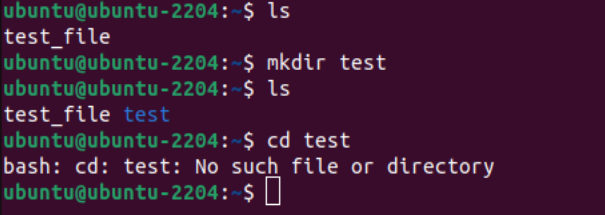
\includegraphics[width=1\linewidth]{bilder/attacker.png}
    \caption{Attacker's perspective: Attempt to change into a fake directory fails.}
\end{figure}

In contrast, the honeypot's logs accurately reflect the expected behavior within the simulated environment. These logs confirm that the directory change would have been successful if it had been handled entirely within the honeypot. The logs include details about the intercepted \texttt{chdir()} system call, the target directory, and whether the operation was valid. The screenshot below shows the corresponding log entry:

\begin{figure}[H]
    \centering
    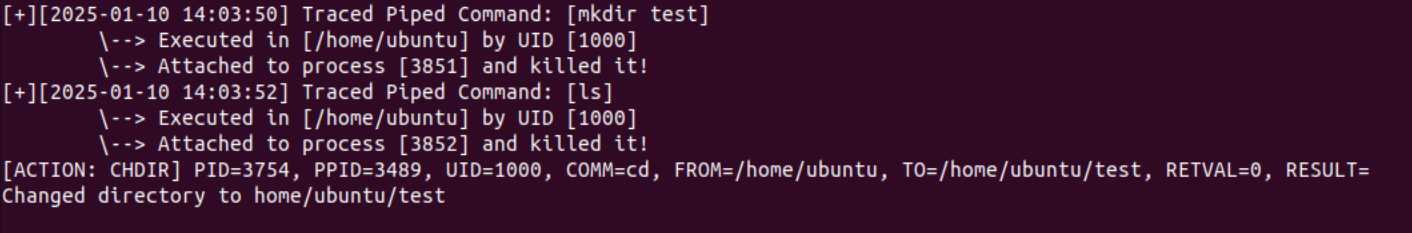
\includegraphics[width=1\linewidth]{bilder/logs.png}
    \caption{Honeypot logs: Successful directory change simulation.}
\end{figure}

This example highlights the current limitation of executing \texttt{cd} on the host system rather than fully within the honeypot and demonstrates how the extended eBPF code and logging provide accurate simulation data for future enhancements.

\subsection{Piped Commands}
\label{sub:pipes}

The goal of implementing piped commands in the honeypot was to simulate Linux-like behavior when executing multiple commands chained together using the pipe symbol (\texttt{|}). However, due to the nature of how piped commands operate and the honeypot's current architecture, several challenges arose, requiring additional analysis and foundational improvements for future enhancements.

Piped commands execute each command in the chain as a separate process, with the output of one command serving as the input to the next. For example, a command like \textbf{\texttt{touch test | ls}} spawns two distinct processes:

\begin{enumerate}
    \item \texttt{touch test}, which creates a file named \texttt{test}.
    \item \texttt{ls}, which lists the contents of the directory, including the newly created \texttt{test} file.
\end{enumerate}

The pipe ensures that the output of the first process (\texttt{touch test}) is directly connected to the input of the second process (\texttt{ls}). This sequential data flow makes it difficult to handle piped commands in the honeypot, as the current implementation processes one command at a time without considering the interdependence of outputs and inputs in a pipeline.

Using \texttt{strace}, the behavior of piped commands was analyzed. The command produced output revealing a \texttt{pipe2} system call, which is used to establish the communication channel between commands in the pipeline:

\begin{lstlisting}
$ strace -f bash -c "touch test | ls"
... 
pipe2([3, 4], 0)                   = 0
... 
\end{lstlisting}

This discovery highlighted that the honeypot needed to intercept \texttt{pipe2} system calls in addition to the existing \texttt{execve} monitoring. To address this, the eBPF code was extended as follows:

\begin{lstlisting}
int syscall__pipe2(struct pt_regs *ctx, int __user *pipefd)
{
    struct data_t data = {};
    u32 uid = bpf_get_current_uid_gid() & 0xffffffff;
    if (uid != UID_FILTER) {
        return 0;
    }

    data.pid = bpf_get_current_pid_tgid() >> 32;
    data.uid = uid;
    data.timestamp = bpf_ktime_get_ns();
    bpf_get_current_comm(&data.comm, sizeof(data.comm));
    data.type = EVENT_PIPE;
    events.perf_submit(ctx, &data, sizeof(data));
    return 0;
}
\end{lstlisting}

This enhancement enabled the honeypot to detect when a pipeline was initiated, allowing further logic to handle piped commands.

Despite detecting the \texttt{pipe2} system call, several challenges remained:

\begin{enumerate}
    \item Command Sequencing: Since each command in the pipeline spawns a separate process, there is no straightforward way to determine the total number of commands in the pipeline or their exact order. The \texttt{execve} calls are processed one by one, meaning the honeypot would process and output each command individually, breaking the sequential flow required for a proper pipeline simulation.

    \item Simulating Outputs and Inputs: The honeypot needs to store the output of each command in the pipeline and pass it as input to the next. Initially, a \texttt{piped} flag was introduced, which, when set to \texttt{True}, prevented the immediate output generation. Instead, command outputs were temporarily stored in a buffer. The idea was to wait until the final command in the pipeline was reached before processing the output.

    \item Identifying the Final Command: A significant challenge was determining when the last command in the pipeline had been reached. Since the honeypot processes each \texttt{execve} call independently, there was no clear indicator marking the end of the pipeline. The \texttt{pipe2} system call does not provide information about how many commands are connected via pipes. To address this, a counter was implemented to track the number of commands. For simplicity, an initial predefined maximum of two commands was set, and once this limit was reached, the pipeline processing logic was triggered.

    \item Re-execution and Ordering: Another approach involved collecting all processes in the pipeline, sorting them for example by process ID (PID) to ensure the correct order, and then re-executing the commands in sequence. This method faced issues as many processes had already terminated by the time the re-execution logic was applied, making it impossible to write outputs back to their respective \texttt{/proc/<pid>/fd/1} files.
\end{enumerate}

The current implementation focuses on handling up to two commands in a pipeline. Outputs are buffered, and the pipeline's results are written to the final process in the chain. However, due to the nature of piped commands and the limitations of the current architecture, several issues persist:

\begin{itemize}
    \item Processes often terminate too quickly, making it almost impossible to reliably attach to them using \texttt{attach\_trace}. As a result, capturing their outputs or integrating them into the pipeline simulation frequently fails.
    \item The reordering of processes is error-prone and does not always align with real-world behavior.
    \item Simulating complex pipelines with more than two commands remains infeasible due to these challenges, as the current implementation struggles to handle interdependent processes in a coordinated manner.
\end{itemize}

The earlier approach of re-executing all processes in the correct order would theoretically allow the honeypot to handle pipelines with an arbitrary number of commands. However, due to the issues with terminated processes and inaccessible file descriptors, this method was ultimately abandoned in favor of the simpler two-command limit.

Due to these challenges, parts of the code have been commented out and are currently non-functional. These sections, however, serve as a foundation for future improvements. They highlight key areas where the logic could be refined to achieve a more reliable and accurate simulation of piped commands. While the current logic is not yet robust enough for consistent and trustworthy results, it provides valuable insights and a framework for developing a fully functional implementation.

\subsection{iptables}
\label{sub:iptables}

The \texttt{iptables} command simulates the basic functions of the Linux command \texttt{iptables}, which makes it possible to use network filters. Therefore, a central class, Iptables, is used to manage and store the groups (chains) and the related rules. The predefined chains in this implementation are INPUT, FORWARD, and OUTPUT. These chains are managed by a class located in the helper folder, specifically in the \texttt{iptable.py} file. This class is designed to efficiently handle the storage, retrieval, and management of rules.

The class contains the following functions:

\begin{itemize}
    \item add\_rule(self, chain, source, destination, protocol, source\_port, destination\_port, action): This function makes it possible to create new rules for the various chains.
    \item remove\_rule(self, chain, source, destination, protocol, source\_port, destination\_port, action): This function allows you to delete certain rules.
    \item list\_rules(self): This function lists all existing rules together with their chains.
    \item clear\_chain(self, chain): This function can be used to empty a chain.
    \item clear\_all(self): This function can be used to remove all existing rules.
    \item rule\_exists(self, chain, source, destination, protocol, source\_port, destination\_port, action): This function can be used to check whether a specific rule exists or not.
\end{itemize}

It supports various arguments like -L, -h, -help, -A, -D and -F. The functions of these arguments are explained below:

\begin{itemize}
    \item -L: This argument allows you to output the current rules and chains.
    \item -h \& –help: This argument can be used to output the help overview.
    \item -A: This argument can be used to create a new rule.
    \item -D: This argument allows you to delete a rule. It checks whether the rule to be deleted does exists.
    \item -F: With this argument, either all chains or only a specific chain can be emptied by passing a chain name.
\end{itemize}

For example you can display all chains and rules with the command \textbf{\texttt{iptables -L}}:

\begin{figure}[H]
    \centering
    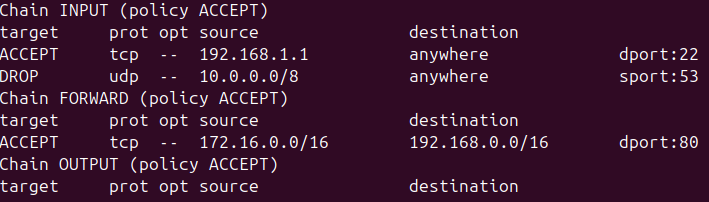
\includegraphics[width=1\linewidth]{bilder/output-iptables.PNG}
    \caption{iptables output}
\end{figure}

To block outgoing ICMP traffic and prevent pings, you can use the following approach:

For example, executing the command \textbf{\texttt{iptables -A OUTPUT -p icmp -j DROP}} will add a rule to the OUTPUT chain that blocks all outgoing ICMP packets. As a result, if you try to ping a domain, like ping google.com, the request will fail because the ICMP packets are dropped.

\begin{figure}[H]
    \centering
    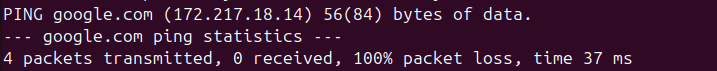
\includegraphics[width=1\linewidth]{bilder/ping_fail.PNG}
    \caption{ping fail}
\end{figure}

\subsection{cat}
\label{sub:cat}
The \texttt{cat} command replicates the core functionality of the Linux \texttt{cat} command, enabling the content of a file to be displayed directly in the terminal. In this implementation, simulated files and their contents are represented as file objects created using the touch command. The contents of each file are stored in the file\_content variable within the corresponding class, ensuring efficient access and management of file data.

When executing the \texttt{cat} command, the process begins by checking whether a file name has been provided as an argument. If an argument is supplied, the command then verifies whether the specified file exists. Once confirmed, it determines if the argument refers to a file or a folder. If the argument equals a folder, an error message is displayed, indicating that directories cannot be processed. However, if the argument corresponds to a valid file, the command reads and displays its content directly in the terminal.

For instance, if you use the \texttt{cat} command to display the contents of a script, the output will show the file's text as follows:

\begin{figure}[H]
    \centering
    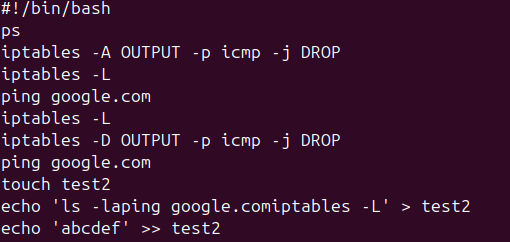
\includegraphics[width=1\linewidth]{bilder/cat.PNG}
    \caption{Simulated output of cat command}
\end{figure}

\subsection{bash}

The bash(self, args, scr\_dir) function provides the capability to execute scripts with various contents in a secure and controlled environment. To run a script, the command \textbf{\texttt{./{filename}}} is used. When executed, the function first checks whether the specified file exists. If the file is not found, an appropriate error message is displayed. However, if the file exists, the function verifies whether it is an executable file and whether the required permissions are in place for execution.

If the necessary permissions are granted, the script's execution begins. The script's content is processed line by line, with each line sent for execution individually. If the first line of the script contains a shebang (e.g., \#!/bin/bash), it is recognized and skipped to prevent errors during execution. Once the shebang is processed, each command in the script is passed sequentially to the execute\_command(self, command, src\_dir) function, which is placed in the \texttt{scripts.py} file within the helper folder. This modular approach ensures a robust and error-free execution of scripts.

Additionally, commands like \texttt{echo} can include text inside quotation marks (' or "), which might contain line breaks. These line breaks are treated as part of the text, and everything inside the quotation marks is processed as a single unit to avoid errors.

\begin{figure}[H]
    \centering
    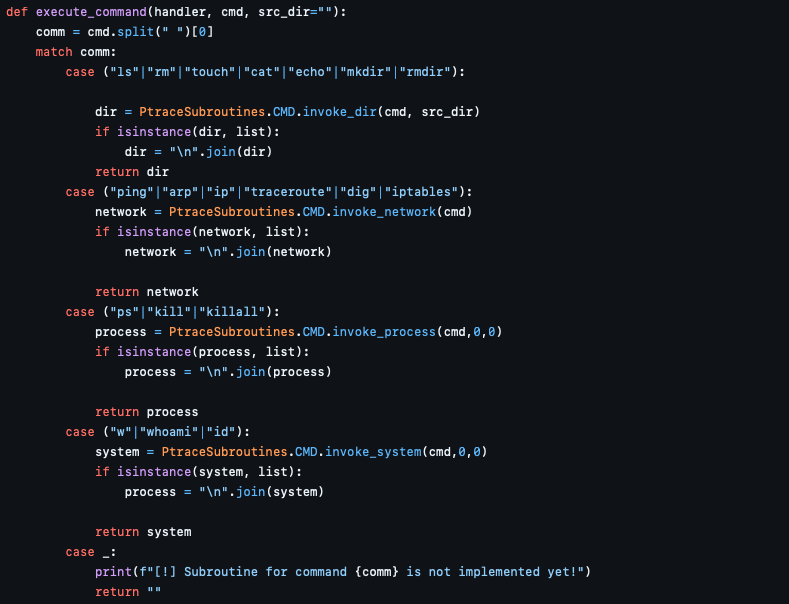
\includegraphics[width=1\linewidth]{bilder/execute_command.PNG}
    \caption{Execute Command function}
\end{figure}

The execute\_command function is designed to process individual commands without creating a separate process, returning the result of each command as a string. These output strings are collected by the bash function, merged into a single output, and then displayed in the terminal.

The execute\_command function takes two arguments: cmd (the command to execute) and an optional src\_dir (the source directory, if required). The function operates by analyzing the main command (the first part of cmd), identified by splitting the string at the first space. Based on this, the command is routed to the right subroutine corresponding to its type. This makes sure that each command is handled properly and efficiently, and its output is combined smoothly into the final result provided by the bash function.

For example, if you execute a script that has the following content:

\begin{lstlisting}
#!/bin/bash
iptables -A OUTPUT -p icmp -j DROP
iptables -L
ping google.com
iptables -D OUTPUT -p icmp -j DROP
iptables -L
ping google.com
\end{lstlisting}

The individual commands are executed sequentially. First, a new iptables rule is added to block all ICMP packets. Afterward, the current iptables rules are listed to confirm that the new rule has been successfully created. Next, a ping to google.com is attempted, demonstrating that the rule is functioning correctly by dropping the ping request. Finally, the rule is removed, the updated rules are displayed, and a subsequent ping is performed to verify that ICMP traffic is working again.

The output appears as follows:

\begin{figure}[H]
    \centering
    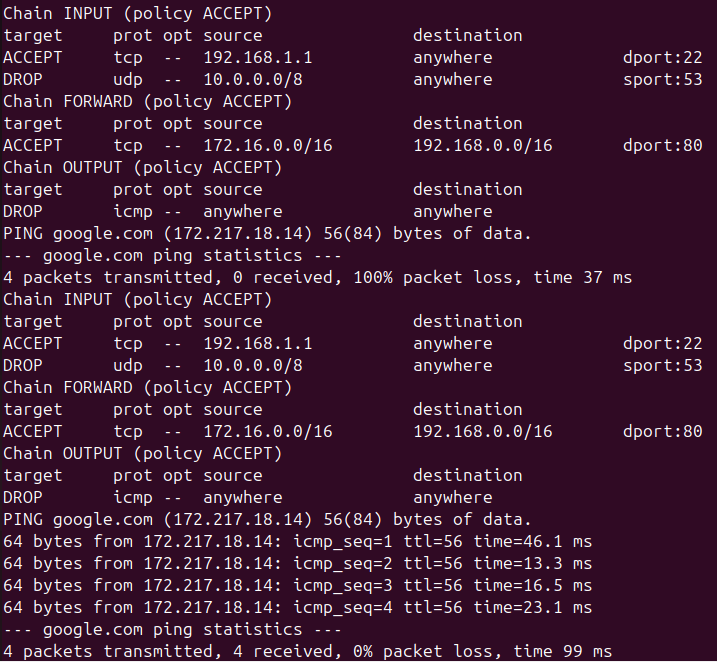
\includegraphics[width=1\linewidth]{bilder/script.PNG}
    \caption{Simulated output of "script"}
\end{figure}

\subsection{echo}
\label{sub:echo}
The \texttt{echo} command is not fully implemented as it is a shell build-in command by default. Built-ins are processed directly by the shell itself and are not executed as independent executable files in the file system. That's why the \texttt{echo} command does not work completely. 
In contrast, /bin/echo works because it is an independent executable file that is located directly in the file system. When using /bin/echo, a new process is started that executes system calls such as execve, allowing the command to be monitored and traced. However, using only \texttt{echo} results in the shell's built-in being executed, which is processed internally and does not generate comparable system calls.

If the \texttt{echo} command is implemented in a script, the built-in echo also works reliably. This is because executing the bash function simulates the individual commands within the script without creating a process.

The echo function starts with a check of the arguments (args). If no arguments are specified, a line break (\textbackslash n) is simply returned, as is the case with the original \texttt{echo} command.

It is then checked whether redirection characters such as \texttt{>} or \texttt{>>}  are contained in the arguments. If no redirection is specified, the function simply returns the arguments as a linked string. If redirection characters are found, the function attempts to write the text to the specified file. If one of these arguments is found, the function checks if the target file exists. If the file exists, the new text is written to the contents of the file. If the file does not exist, the function returns an error message: \texttt{-bash: ‘\{target\_file\}’: No such file or directory}.

\begin{figure}[H]
    \centering
    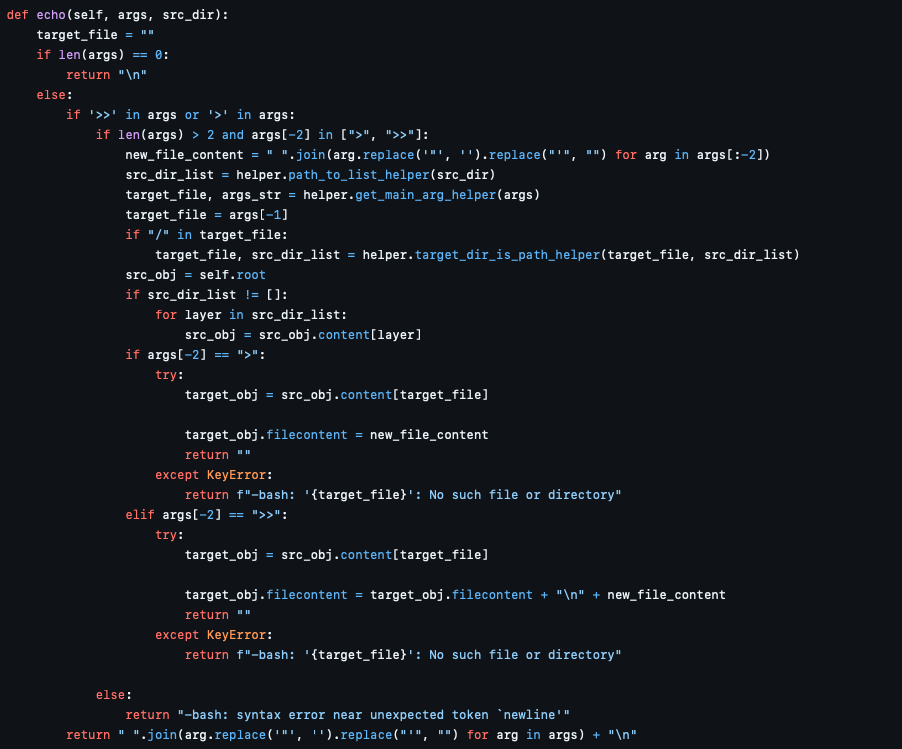
\includegraphics[width=1\linewidth]{bilder/echo_code.PNG}
    \caption{Echo function}
\end{figure}

Problems:

During development, problems often occurred with the ptrace call. A common issue was the error \texttt{No such process}, which appeared when trying to trace a process.

\begin{figure}[H]
    \centering
    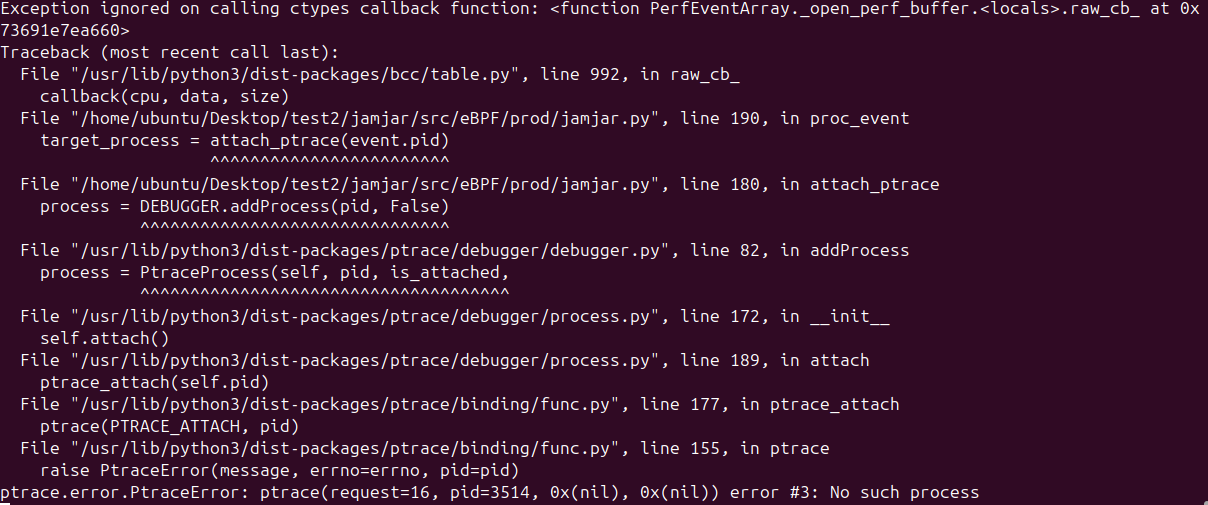
\includegraphics[width=1\linewidth]{bilder/error.PNG}
    \caption{error}
\end{figure}

After analyzing this error, we quickly came to the conclusion that the problems were caused by the short lifespan of the processes. Probably the processes are terminated too quickly so that the ptrace call can no longer be called in time. To check this, we adapted the attach\_ptrace function that throws the error and added some checks:

\begin{figure}[H]
    \centering
    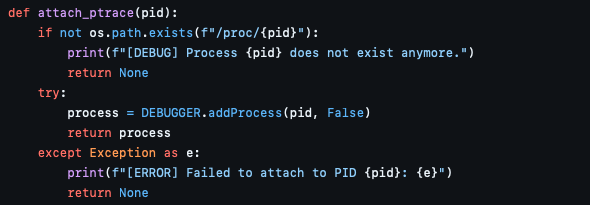
\includegraphics[width=1\linewidth]{bilder/attach_ptrace.PNG}
    \caption{ptrace function}
\end{figure}

This checks whether the process to be terminated still exists at the time of the attach\_ptrace call. If it no longer exists, a suitable message is displayed in the console. If the process is found, the attach\_ptrace function is processed normally.

The results of this adjustment confirmed the assumption, as in some cases the process no longer existed at the time of the attach\_ptrace call.

\begin{figure}[H]
    \centering
    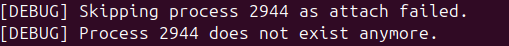
\includegraphics[width=1\linewidth]{bilder/skipping.PNG}
    \caption{ptrace error}
\end{figure}